\documentclass{article}
\usepackage[utf8]{inputenc}
\usepackage[margin=1.0in]{geometry}
\usepackage{graphicx}
\usepackage{wrapfig}
\usepackage{amsmath}
\usepackage{subfig}
\usepackage[makeroom]{cancel}
\let\vec\mathbf
\usepackage{float}

\title{Image Matting and Composting}
\author{Neal Bayya }
\date{May 2019}

\begin{document}

\maketitle

\section{Introduction}
Image matting is the process of separating a foreground object out of one image and composting is the process of pasting it against a new background. It is commonly used in films to composite an actor in a computer-generated scene. The most common form of matting in TV studios and movies is blue screen matting. Techniques exist for segmenting objects in an image (namely GrabCut segmentation, snakes, and scissors) often provide coarse boundary lines which make the object look as it it is super-imposed on the background.  

\begin{figure}[h]
 \centering
 \subfloat{{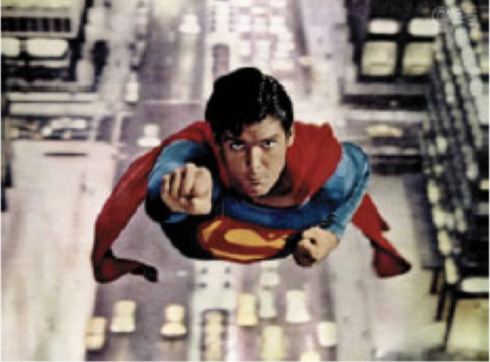
\includegraphics[]{matting_intro.png}}}
 \label{superman}
 \caption{Matting and Composting in Film}
\end{figure}

\section{$\alpha$-matted color images \& Compsoting}

\begin{figure}[h]
 \centering
 \subfloat{{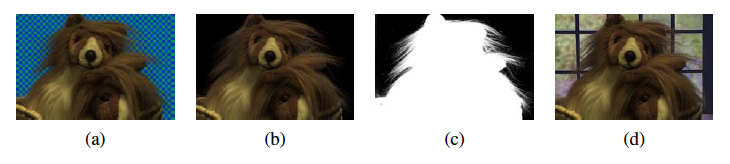
\includegraphics[]{alphamatting.png}}}
 \caption{(a) Source Image; (b) extracted foreground object F; (c) alpha-matte $\alpha$ in greyscale; (d) new composite C}
 \label{alphamatting}
\end{figure}

The intermediate representation for the foreground object in Figure \ref{alphamatting}c is called the \textit{alpha-matted color image}. In addition to the 3 color channels (R, G, and B), $\alpha$-matted images have an $alpha$ channel which quantifies the opacity at each pixel. Pixels which are fully transparent have an $\alpha$ value of 0 and those that are fully opaque will have an $\alpha$ value of 1. For example, the image in Figure \ref{alphamatting}c is completely opaque at pixels which are inside the stuffed animal and transparent elsewhere. A natural question arises: when would you have an $\alpha$ value that is not binary? Pixels that lie on the boundary of objects often have varying $\alpha$ values. Additionally, motion blur causes non-binary $\alpha$ values. \\
To composite a foreground image onto an old background image, the following composting equation is used:
\begin{equation*}
    C = (1-\alpha) B + \alpha F
\end{equation*}
where B is the background image and F is the foreground image. Intuitively, the foreground should have more influence (and background less) in the resulting image if regions of higher opacity. Convince yourself that the compositing equation obeys such intuition.  \\


\section{Matting}
We can quickly see that image matting is a much more difficult process than image composting. More formally, image matting consists of taking the image C and decomposing it into a background image (B), a foreground image (F), and a map of $\alpha$ values. 

\begin{eqnarray*}
C_r &=& \alpha F_r  + (1-\alpha) B_r \\
C_g &=& \alpha F_g  + (1-\alpha) B_g \\
C_b &=& \alpha F_b + (1-\alpha) B_b 
\end{eqnarray*}

The equations shown above demonstrate the difficulty of the problem. We have 3 equations and 7 unknowns ($\alpha$, $F_r$, $F_g$, $F_b$, $B_r$, $B_g$, $B_b$.

\subsection{Blue-screen matting}
In traditional blue-screen matting, we assume that the foreground has no blue and the background is mainly comprised of blue. Ideally, $F_b = 0$, meaning that there is absolutely no component of blue in any object in the foreground image. Likewise the blue background constraint allows us to say that $B_r = B_g = 0$. As a result, our equations simplify to 
\begin{eqnarray*}
C_r &=& \alpha F_r  \\
C_g &=& \alpha F_g  \\
C_b &=& (1-\alpha) B_b 
\end{eqnarray*}

\begin{figure}[t]
 \centering
 \subfloat{{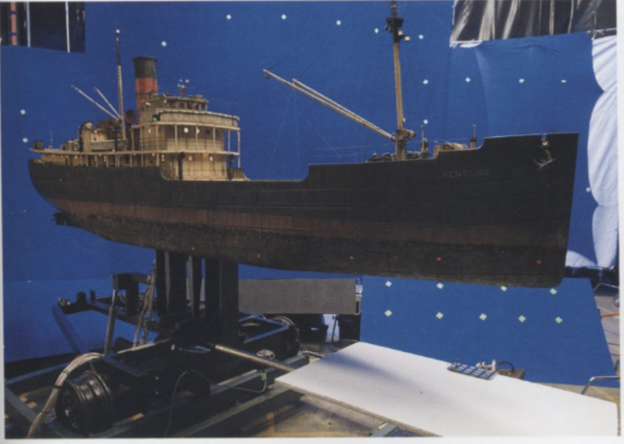
\includegraphics[]{blue.png}}}
 \label{superman}
 \caption{Blue-screen matting}
\end{figure}

This simplified model gives us 3 equations and 3 knowns, which we can solve.

\subsection{Generalize a bit}
Now, let's assume that there is a grey object in the foreground image. Let's keep the constraint that the background image is completely blue ($B_r = B_g = 0$). Since we know that grey is formed by equal quantities of red, green, and blue, we can add the constraint: $F_r = F_b = F_g = F$. Our equations then become:
\begin{eqnarray*}
C_r &=& \alpha F  \\
C_g &=& \alpha F  \\
C_b &=& \alpha F + (1-\alpha) B_b 
\end{eqnarray*}

A similar simplification can be made with skin color because we can model the foreground color as $F = \left(k, k/2, k/2\right)$.

\textbf{Issues with blue screen matting}: 
\begin{enumerate}
    \item Blue-eyed people will not be able to be in the foreground because the foreground may not have any pixels which are dominated by blue.
    \item The blue background will illuminate the foreground, so we will typically see the foreground image surrounded by a blue silhouette after it is composted. The only solution to this is to modify the blue channel.
    \item The foreground may cast shadows onto the blue background.
\end{enumerate}

\section{Challenge}
Think of some constraints you could add to the foreground and background to matte various objects. [Hint: Multiple images against different background colors.]
\end{document}
